\documentclass[11pt]{amsart}
\usepackage{amsfonts}
\usepackage{amsmath}
\usepackage{amsthm}
\usepackage{graphicx}
\usepackage{amssymb}
\usepackage{mathrsfs}
\usepackage[numbers]{natbib}
\usepackage[fit]{truncate}


\newcommand{\truncateit}[1]{\truncate{0.8\textwidth}{#1}}
\newcommand{\scititle}[1]{\title[\truncateit{#1}]{#1}}

\pdfinfo{ /MathgenSeed (169491006) }

\theoremstyle{plain}
\newtheorem{theorem}{Theorem}[section]
\newtheorem{corollary}[theorem]{Corollary}
\newtheorem{lemma}[theorem]{Lemma}
\newtheorem{claim}[theorem]{Claim}
\newtheorem{proposition}[theorem]{Proposition}
\newtheorem{question}{Question}
\newtheorem{conjecture}[theorem]{Conjecture}
\theoremstyle{definition}
\newtheorem{definition}[theorem]{Definition}
\newtheorem{example}[theorem]{Example}
\newtheorem{notation}[theorem]{Notation}
\newtheorem{exercise}[theorem]{Exercise}

\begin{document}


\begin{abstract}
 agregar un abstract 
\end{abstract}


\scititle{Informe del Proyecto Final del curso Fundamentos Matemáticos del procesamiento de señales, Síntesis de sonidos Percusivos}
\author{K. Diaz Torres}
\date{26-01-2022}
\maketitle











\section{Introducción}

 En este proyecto trabajaremos con sonidos del tipo percusivo, un sonido percusivo será aquel que es producido por la vibración libre de una estructura o un medio que ha sido puesto en movimiento por algún tipo de excitación. Por ejemplo: Batería, vibráfono, marimba, campana, triángulo, piano, guitarra, etc. Además de esto es necesario saber que los sonidos percusivos se pueden descomponer principalmente en dos partes consecutivas:\\
\begin{itemize}
\item El ataque (Sonido inicial y de corta duración): Es el resultado inicial de golpear/perturbar algún material resonante. Esta parte del sonido tiene una estructura compleja bastante difícil de analizar, modelar o sintetizar. 
\item La resonancia (Sonido final y decreciente): Es el resultado de la estabilización del medio, es decir, el proceso en el que pasa de vibrar mucho a casi no vibrar. El sonido generado por la resonancia se puede modelar con sinusoides amortiguadas exponencialmente.
\end{itemize}
 En este proyecto nos centraremos en la parte del ataque. Utilizando Modelos de filtrado y excitación.



\section{Modelo de excitación simple/Modelo de filtrado.}
Los filtros resonantes a utilizar: para un $z$,
$$
H(z)=\frac{B(z)}{A(z)}, \ \ \text{ con,}
$$
$$
B(z)= \prod_{i=1}^{q}(1-w_iz^{-1}), \ \ \text{ y,}
$$
$$
A(z)=\prod_{i=1}^{p}(1-z_iz^{-1}).
$$
De donde $A$ y $B$ son polinomios en la variable compleja $z^{-1}$. Además los complejos $z_i$ y $w_i$ son los ceros y polos de la función $H(z)$. Para efectos de estabilidad requerimos que los polos $z_i$ vivan dentro del círculo unitario $|z_i|<1$. \\
La frecuencia $f_i$ y el factor de amortiguamiento $\alpha_i$ están dados por,
\begin{eqnarray}
f_i=\dfrac{F_s}{2 \pi} arg(z_i), \ \ \text{ y }, \\
\alpha_i = -F_s \log(|z_i|).
\end{eqnarray}
De donde el valor $F_s$ denota la frencuencia de muestreo de la señal. Revisemos algunos filtros.
\subsection{Filtro de todo los polos.}
Si $B(z)=1$, el filtro $H(z)$ es un filtro de todos los polos tal que,
$$
H_{a\ p} (z) = \prod_{i=1}^{p} \dfrac{1}{1-z_iz^{-1}}
$$
Dado que $H_{a \ p}$ no tiene zeros,es un filtro de fase mínima. Es decir la inversa es un filtro casual y estable.
\subsection{Sección paralela del seno de segundo orden.}
En este caso el filtro es,
$$
H_{sc}(z)=\sum_{i=1}^{p/2} \dfrac{j}{1-z_iz^{-1}}+\dfrac{-j}{1-\overline{z_i}z^{-1}}
$$
Este filtro está compuesto por un conjunto de secciones de segundo orden reales en paralelo.
\subsection{Sección paralela del coseno de segundo orden.}
En este cas  consideramos $B$ tal que,
$$
B(z) = \sum_{i=1}^p \prod_{j \neq i} (1-z_jz^{-1}),
$$
y luego el filtro queda,
$$
H_{cc}(z) = \sum_{i=1}^{p} \dfrac{1}{1-z_iz^{-1}}
$$
De donde en este caso la inversa también es un filtro casual y estable. Y $H_{cc}$ está compuesto por un conjunto de secciones de segundo orden en paralelo.
\section{Modelo de excitación simple/Modelo de múltiple filtrado.}
En esta parte se asume que tenemos un conjunto de sonidos $s_n^i$ que corresponden al mismo instrumento percutado de la misma manera.
En este modelo asumiremos la existencia de una sola señal de excitación $e(n)$ y un conjunto de filtros resonantes $H_i$, tales que todos los sonidos originales pueden ser sintetizados utilizando la misma señal de excitación en cada uno de los filtros resonantes. \\
\begin{figure}
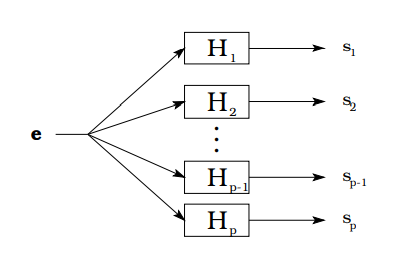
\includegraphics[scale=1]{grafo1.png}
\end{figure}
\\
Sin embargo conseguir sonidos correspondientes de la misma señal de excitación no es algo fácil de poner en práctica, más adelante mencionaremos una forma de hacerlo. \\
\section{Estimación de los parámetros.}
\subsection{Estimación del filtro resonante.}
Como el filtro $B(z)$ es arbitrario, solo estimaremos el filtro $A(z)$. Por lo que asumiremos 
Los filtros resonantes $H_i$ usados en este modelo son como los vistos anteriormente, es decir, $H_i(z)=B_i(z)/A_i(z)$. De donde $A_i$ dependerá de las frecuencias y los factores de amortiguamiento de las sinusoides de las partes decrecientes de las señales $s_i$ y por otro lado $B_i$ serán escogidos de manera arbitraria. Supondremos además que tenemos una señal percusiva original $s$ que intentaremos modelar como la salida de un filtro resonante alimentado por una señla de excitación de corta duración. Además de (1) y (2), tenemos las relaciones entre los zeros de $A(z)$ y las frecuencias $f_i$ y los factores de amortiguamiento.\\ \\
 Primeramente el espectro de potencia $P_i(f)$ sucesivos se calculan en una ventana situada en tiempos crecientes $n_i$. Estos espectros luego se acumularan partiendo desde el último hasta el primero. Este procedimiento produce un espectro de potencia 3D, tal que así
\begin{eqnarray}
P_{cum}(f,i)=\log\left[\sum_{k \geq i} |P_k(f)|^2\right], \ \ \text{ con, } \\
P_i(f)=\sum_{k=0}^{N-1}s_{k+n_i}w_k e^{-j2\pi k f /N}.
\end{eqnarray}
Donde los $w_k$ representan una ventana de ponderación, usualmente una ventana de Hamming. Y $P_{cum}(f,i)$ es el valor en la frecuencia $f$ del espectro acumulado sobre el rango $k\geq i$. \\ \\
En segundo lugar, detectamos el pico (el peak) en el espectro de potencia acumulada $P_{cum}(f,1)$ para detectar los componentes sinusoidales y calcular su frecuencia. Se pueden tener estimaciones precisas usando una interpolación de segundo grado. \\ \\
Finalmente los factores de amortiguamiento son estimados a partir de la pendiente del espectro de potencia 3D, cuando $f$ se mantiene constante e $i$ varía. Como los espectros de potencia no son negativos, la acumulación hacía atrás hace que el \textit{alivio del deterioro de la energía} sea una función decreciente en el tiempo para cualquier frecuencia dada. Una vez los valores de las frecuencias modales y los factores de amortiguamiento son estimados, los polos $z_i$ se estiman de las ecuaciones (1) y (2). Finalmente para $A(z)$ usamos que
$$
A(z)=\prod_{i=1}^{p}(1-z_iz^{-1}).
$$
\subsection{Estimación de la señal de excitación para el Modelo de excitación simple/Modelo de filtrado.}
Ahora que tenemos estimado $A(z)$ y dado la elección de$B(z)$ el cálculo del filtro de excitación es un clásico problema de filtrado inverso. Este problema tiene algunas similitudes con el LPC (codificación de predicción linear). Dos implementaciones se pueden utilizar para estimar la señal de excitación.

\subsubsection{Filtrado inverso con dominio en el tiempo} Consiste en filtrar la señal original con la inversa de $H(z)$,
$$
H^{-1}(z)=\dfrac{A(z)}{B(z)}
$$
Existen problemas con esto asociados a los zeros de $B$. \\
\begin{itemize}
\item \textbf{Problema de estabilidad de $H^{-1}(z)$:} Si $B(z)$ tiene zeros fuera del circulo unitario entonces $H^{-1}(z)$ es inestable y por lo tanto un filtro inverso no puede ser aplicado directamente. Una de las soluciones es separar $B(z)$ en una parte de fase mínima $B_{min}(z)$ y una parte de fase máxima $B_{max}(z)$. En donde $B_{min}(z)$ corresponde a la parte en donde están las raíces dentro del círculo unitario y $B_{max}(z)$ a las que están fuera. La señal $s_n$ es filtrada por $A(z)$, entonces por $1/B_{min}(z)$ en donde el resultado es en tiempo reverso. El filtro $1/B_{max}(z)$ se convierte en el de fase mínima reflejando sus raíces dentro del círculo unitario, lo que es equivalente a leer sus coeficientes hacía atrás. Este filtro es utilizado para procesar la señal en tiempo reverso obtenida del paso anterior. Finalmente el resultado es el tiempo invertido para producir la señal de excitación $e_n$. Todo este proceso puede ser evitado escogiendo un filtro de resonancia que es de fase mínima, como lo es en el caso del filtro de todos los polos y en el filtro de sección paralela coseno-seno de segundo orden.
\item \textbf{Problema de mal planteamiento por la naturaleza de un filtro inverso:} Dado que Excitaciones muy diferentes pueden dar resultados similares en el sentido de la norma $L^2$, despues de filtrar por $H(z)$; podemos tener un problema de mal planteamiento  y encontrar una señal de excitación errónea. Equivalentemente, las señales $e_n$ correspondientes a dos señales muy similares $x_n$ pueden ser extremadamente diferentes y de hecho esto es algo que no queremos.
\item \textbf{Mal acondicionamiento de los coeficientes del filtro:} $A(z)$ fue determinado con los valores de sus raíces; expresar $A$ como un polinomio, puede hacer que tengamos coeficientes muy largos, especialmente si sus raíces están muy cercas unas de otras. Dándonos problemas series en cuando a computo se refiere.
\end{itemize}
\subsubsection{Deconvolución con dominio en la frecuencia.}
Con ciertas precauciones podemos plantear el dominio en la frecuencia utilizando la Transformada de Fourier discreta. Es bien sabido que la la convolución circular de dos señales $u_n$ y $v_n$ puede ser calculada multiplicando sus Transformadas de Fourier discretas complejas $U_k$ y $V_k$ respectivamente y tomando la inversa. De donde la mayor ventaja de este esquema es el poder utilizar la Transformada de Fourier Rápida. Una condición suficiente para que la convolución circular sea equivalente a una convolución acíclica es que la longitud de la DFT, digamos $N$ tiene que satisfacer,
$$
N > N_u+N_v-1
$$
donde $N_u$ y $N_v$ denota la longitud de las dos señales $u_n$ y $v_n$ respectivamente. En otras palabras, la longitud $N$ de la DFT tiene que ser mayor que la longitud de la señal $u \star v$, donde $\star$ denota la convolución acíclica. \\ Se sigue que la deconvolución con dominio en la frecuencia puede ser estimada utilizando la DFT: la DFT de la señal original $x_n$ y de la respuesta de impulso $h_n$ del filtro $H(z)$ son calculadas, asegurándonos que se cumplen todas las condiciones establecidas anteriormente. 	Para cada frecuencia discreta, la primera se divide por la segunda y se toma una transformada de Fourier inversa del resultado, lo que da la señal de excitación. La implementación de este proceso tiene menos limitantes que el anterior mostrado, como tal
\begin{itemize}
\item \textbf{Estabilida de $H^{-1}(z)$} Este proceso puede utilizarse aun cuando el filtro $H(z)$ no es de fase mínima y por ende $H^{-1}(z)$ es estable, esto nos evita el proceso de usar un esquema de doble filtro de fases diferentes.
\item \textbf{Problema de planteamiento:} Este problema está expuesto de manera intrínseca, así que no es algo de lo que preocuparse.
\item \textbf{Mal acondicionamiento de los coeficientes del filtro:} Dado que no tendremos que expresar $A$ como un polinomio esto ya no es un problema.
\end{itemize}
Es por todo esto que preferiremos utilizar el método de deconvolución con dominio en la frecuencia.

\subsection{Estimación de la señal de excitación para el Modelo de excitación simple/Modelo de múltiple filtrado.}

\subsubsection{Deconvolución de mínimos cuadrados.} Cuando utilizamos estos modelos el problema de encontrar la señal de excitación corresponde a varios pares de sonidos originales y filtros resonantes, esto ya no admite una solución exacta puesto que hay más ecuaciones que incógnitas. Es por esto que es natural utilizar soluciones del tipo mínimos cuadrados. Podemos plantearlos de la siguiente manera: \\
Dadas $p$ señales originales $x_n^{i}$ ($0 \leq i \leq p$) y $p$ filtros resonantes $H_i$ con un impulso de respuesta $h_n^{i}$ nosotros buscamos la señal de excitación $e_n$ que minimiza el error acumulativo $\xi$ definido como:
$$
\xi=\sum_{i=0}^{p-1}\left( \sum_{k=0}^{N-1}(x_k^{i}-\hat{x}_k^{i})^2 \right)
$$
con $\hat{x}_k^{i}=h_k^{i} \star e_k$ y $u \star v$ la convolución de dos señales. Es decir el error acumulativo $\xi$ es la suma de los errores cuadrados entra la señal original $x_n^{i}$ y su versión sintética $\hat{x}_n^{i}$. Pero del Teorema de Parseval podemos escribir $\xi$ como
$$
\xi=\int_{-\frac{1}{2}}^{-\frac{1}{2}}\left( \sum_{i=0}^{p-1} | X_i(f)-H_i(f)E(f)|^2\right)df
$$
en donde, $X_i(f)$, $H_i(f)$ y $E(f)$, son las transformadas de Fourier de $x_n^i$, $h_n^i$ y $e_n$ respectivamente. Ahora minimizar la integral que define a $\xi$ es equivalente a minimizar el integrando con respecto a $E(F)$ para cada valor de $f$:
$$
\min_{E(f)}\sum_{i=0}^{p-1}|X_i(f)-H_i(f)E(f)|^2
$$
De donde ahora esto es un minimización cuadrática estándar cutyas soluciones está dada por 
$$
\sum_{i=0}^{p-1}(H_i^*(f)(X_i(f)-H_i(f)E(f)))=0
$$
o que es equivalente
$$
E(f)=\dfrac{\sum_{i=0}^{p-1}H_i^*(f)X_i(f)}{\sum_{i=0}^{p-1}H_i^*(f)H_i(f)}
$$
La señal de excitación con dominio en el tiempo es finalmente obtenida de la Transformada de Fourier inversa. \\ \\
Los problemas:
\begin{itemize}
\item \textbf{Estabilida de los filtros $H_i^{-1}(z)$} 
Como los calculos se están haciendo sobre el dominio de la frecuencia no existen problemas con la estabilidad.

\item \textbf{Problema de planteamiento:} Al utilizar bastantes filtros de resonancia el problema tiende a ser aliviado. Como resultado, parece natural que haya menos "soluciones cercanas" adecuadas.
\item \textbf{Problemas de sincronización:} De existir existen varios métodos para resolver esto, por ejemplo utilizando la técnica de correlación cruzada.
\end{itemize}
\section{Aplicación.}
\subsubsection{Sonidos}
El primer paso fue sencillo, dado que se encontró un pack (los cuales están dentro del repositorio) de sonidos del piano tocados de manera limpia y prolongando la nota durante 10 segundos, es decir, sonidos ideales para el poryecto. Estos estaban en formato .mp3 por lo que se tuvieron que convertir a .wav, además estaban en formato stereo, por lo que a través de la operación
\begin{verbatim}
np.mean(x, axis=1)
\end{verbatim}
\subsubsection{Primeros Problemas Estimando los valores}
El problema principal de esta parte es el tiempo de cálculo, dado que se intentó replicar el algoritmo de forma bruta y no se encontraron formas de optimizarlo, es por estos que al calcular el espectro de potencia acumulada $P_{cum}(f,1)$ se demoró bastante, luego se interpoló y se estimaron los componentes sinusoidales. De donde mis principales dudas se referían a como encontrar las distintas frecuencias propuestas en la ecuación (1). Luego para encontrar los factores de amortiguamiento, se fijó una frecuencia de $f_0=0.5$ y se procedió a calcular $p_{cum}(f_0,i)$ variando el $i$, que por la teoría los factores se obtenían de las pendiente de este espectro obtenido. Cosa que se complico a la hora de intentar plantear un código que rescatase esos valores. \\ \\
Y faltando esta información no se pudieron encontrar los filtros resonantes.
\subsubsection{Problemas Generales}
Básicamente se tuvieron problemas a la hora de implementar el algoritmo al código, y en general se desperdició mucho tiempo intentando replicar el algoritmo de manera bruta y no buscando alternativas más optimizadas, por ejemplo a la hora de definir el $p_{cum}(f,i)$, de la siguiente manera.
\begin{verbatim}
def p(x,f,i):
    ni=7000*i
    Pi=[]
    window=np.hamming(7000)
    for k in range(0,7000):
        Pi.append(x[k+ni]*window[k]*np.exp(-1j*2*np.pi*k*f/7000))
    sumi=sum(Pi)
    return sumi

def pcum(x,f,i):
    accum=[]
    for j in range(0,63-i):
        jaux=62-j
        accum.append(abs(p(x,f,jaux))**2)
    pc=sum(accum)
    return math.log(pc)    
\end{verbatim}
se perdió valioso tiempo a utilizar en poder intentar seguir con el algoritmo, suponiendo un filtro de amortiguamiento cualquiera. \\
Para poder así presentar un código referido a la parte en donde se estima la señal de excitación dado el filtro. \\ 
\section{Conclusión}
En conclusión puedo resumir que en general el proceso del algoritmo lo encontré bastante original y anhelaba poder llegar a obtener dado una señal, los filtros resonantes y la señal de excitación que originó el sonido, para así obtener la síntesis de quizás cualquier sonido del tipo percusivo ingresado al programa. Traté de buscar trabajos similares en la red Github fallando completamente, pero he de admitir que no desistí en intentar hacer surgir ideas y plasmarlas hasta el último día. 





\begin{footnotesize}
\bibliography{scigenbibfile}
\bibliographystyle{plainnat}
\end{footnotesize}

\end{document}
